
\section{ソフト開発の手法}
本研究で開発するソフト"viewer"は,小傾角粒界の原子モデルの配列を2次元で描画する.
viewerは,VASPの入出力で採用されているPOSCAR形式のファイルを読み込んで,原子配列をSVG形式で出力する.
原子配列のSVG表示は,2次元画像描画ライブラリ"rcairo"を用いて作成していく.
それぞれについて,採用したツールや検討した内容について詳述する.

\subsection{一般的な原子モデルソフトとの比較}
結晶描画が可能なソフトとして,"Medea"および"VESTA"がある.
これらは結晶構造や電子・核密度等のデータを読み込んで結晶の形を3次元で可視化できるプログラムである\cite{Vesta}.
これらは原子の配置を確認するために,手作業で結晶構造の視点を自由に変えながら.構造全体を視覚的に理解することができる.図\ref{fig:006}は,VESTAの画面から切り出した原子配置モデルの一例である,3次元に投影することによって得られた図形である.
VESTAの使用には以下の難点があった.

\begin{itemize}
\item 3次元で原子配列を表示するため,各層の原子位置が把握しづらい
\item 色分けするための層を手動でおこなうため,指定した範囲の正確さに欠け,作業に手間がかかる
\end{itemize}
\begin{figure}[htbp]\begin{center}
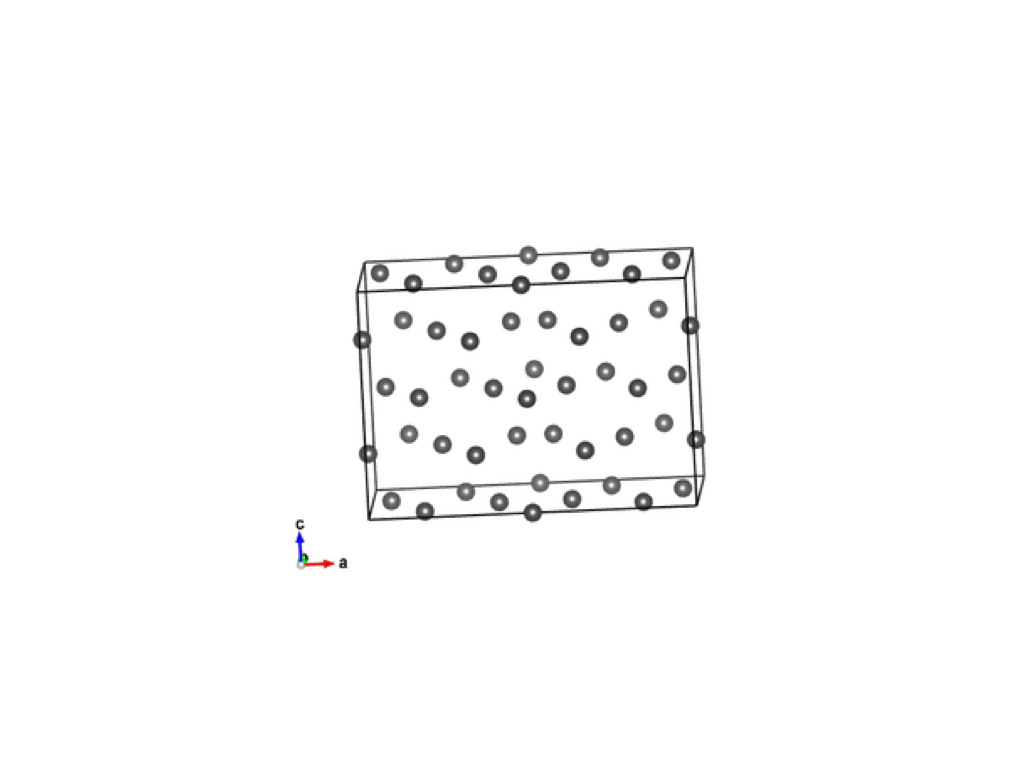
\includegraphics[width=6cm,bb= 0 0 937 753]{../figs/./boundary_narita.006.jpeg}
\caption{VESTAで描画したPOSCAR\_2223の原子配置.}
\label{fig:006}
\label{default}\end{center}\end{figure}
そこで,本研究では,原子配列を多面的に描画した三面図で表示するためのソフト開発を試みた.
三面図を使用して表示することにより,図\ref{fig:007}のように,各面から原子の配置を直感的かつ簡易に確認できるようになる.

\begin{figure}[htbp]\begin{center}
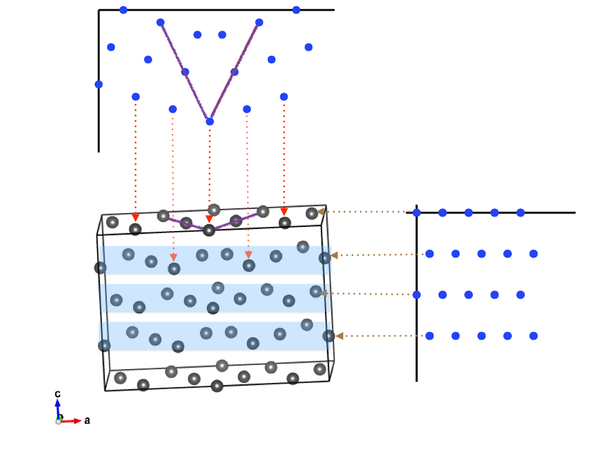
\includegraphics[width=10cm,bb= 0 0 937 753]{../figs/./boundary_narita.007.jpeg}
\caption{vestaの投影図を2次元化した図.}
\label{fig:007}
\label{default}\end{center}\end{figure}
\subsection{MVCモデルの概要と利点}
本研究で開発するソフトは,作業の分業化が容易であるMVCモデルで作成していく.
MVCモデルは,ソフトウェアの設計モデルの一つであり,アプリケーションの開発において取られている手法である.
MVCモデルは図\ref{fig:005}のように三要素で構成されており,データの処理を担う"Model",処理結果を画面に表示する"View",入力情報の受け取って処理機能を制御する"Controller"で設計されている.
各々の機能が直交化されているため,開発作業を分業化しやすく,相互の仕様変更による影響を受けずに開発を進めることが出来る\cite{MVC}.
したがって,原子配列の結果を画面表示する機能構築に特化した開発作業が取り組める.

\begin{figure}[htbp]\begin{center}
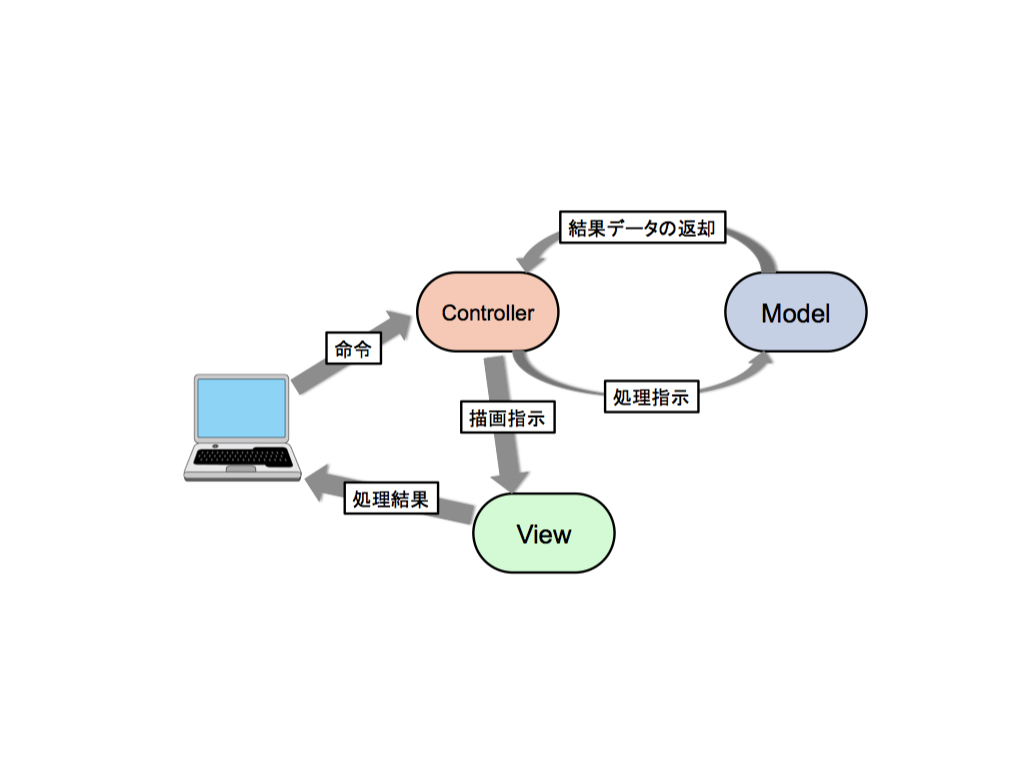
\includegraphics[width=10cm,bb= 0 0 937 753]{../figs/./boundary_narita.005.jpeg}
\caption{MVSモデルの構成と各機能.}
\label{fig:005}
\label{default}\end{center}\end{figure}
\subsection{SVG表示の特徴}
SVGは,XMLを基盤とする2次元画像記述言語であり.イラストレーターで扱うベクターデータである\cite{SVG}.
SVG形式で表示することにより,以下のような利点がある.

\begin{itemize}
\item ベクタ形式で画像を表示するため,曲線や文字の拡大・縮小しても画質が劣化せずに,解像度に応じた出力結果を得ることが出来る.
\item スタイルシートを切り替えることで,特殊な環境下においても目的に応じたグラフィック描画を出力することが可能である
\item テキストデータであるため,テキストエディタやxmlプロセッサを介したファイルの編集が可能である.
\end{itemize}
\subsection{rcairoを使用する利点}
rcairoは,Ruby言語でベクタ形式の2次元描画を容易に実現できるライブラリのことである.
このライブラリは,描画コンテキストを用いたAPIであるため,描画するためのコードを短く簡潔に作成することが出来る.
また.複数の出力をサポートすることができるため,出力先のフォーマットに影響されずに描画処理をおこなうことが可能である\cite{rcairo}.

